\section{Introduction}
\subsection{Purpose of document}
This report documents the contextualization of a problem surrounding the tracking of truckers.
The background and problem is considered, possible solutions with objectives are identified, along with an expected outcome for the potential solution, requirements and scope definition.

The design and implementation of the postulated solution is documented.
Finally, this solution is evaluated and analyzed, and future recommendations are considered.

\subsection{Background}
Due to the nature of the trucking industry, it is difficult for company owners to keep track of their employees.
Truckers carry out their shifts delivering cargo to various locations over far distances.
As such, it is not possible for employers to track their whereabouts throughout their shifts.

Lack of supervision allows truckers the ability to behave undesirably while on the job.
They can waste time by taking unnecessarily long stops.
Some truckers may drive erratically, unsafely or illegally.
Such employees are a liability to the reputation and profitability of their respective companies.

The ability to track truckers would provide a potential means to address this issue, by allowing employers to monitor their truckers' location, progress and behavior throughout their shifts.
The ability to produce an audit trail detailing the truckers whereabouts during their shifts would allow managers to ensure that work is adequately executed. Such an audit trail would comprise of:
\begin{itemize}
\item \textbf{\ac{gps} coordinates\\}
\ac{gps} tracking will allow employers to ensure that truckers are traveling to required locations, and doing so via effective routes. This also allows employers to ensure no unnecessary detours occur.
\item \textbf{Altitude\\}
Altitude logging may be useful for identifying trends in routes traveled, especially where large altitude gradients occur.
Trucks often struggle traversing steep gradients.
Altitude analysis may offer insight for companies looking to perform optimizations.
\item \textbf{Speed\\}
Examining trucker speeds allows for managers to monitor how quickly truckers are able to transport goods.
Slower routes may be identified where traffic is more prevalent.
This could allow for route optimization, or truck malfunctions.
\item \textbf{Acceleration\\}
Acceleration may be used for inferring any dangerous driving behavior. 
Erratic acceleration and deceleration is associated with dangerous driving behavior.
Additionally, erratic driving can cause more strain and deterioration on the vehicle.
\end{itemize}

The ubiquitous nature of cheap, \ac{gps}-equipped smartphones provides a potential avenue for realizing a simple solution at low cost.
In addition, nation-wide continuous access to the internet allows for live tracking to be utilized most of the time.

\subsection{Problem Statement}
A tracking system must be implemented to be used by trucking companies for tracking and logging their truckers' \textbf{\ac{gps} coordinates, altitude, speed and acceleration}.
Logging should be performed with sensors available on most standard smartphones.

Logging data should be continuously (or periodically) made accessible to managers remotely.
In addition, an interface is required for storing, processing and displaying logged data pertaining to the trucker's location and behavior.

\subsection{Hypothesis}
An low-cost anticipated architecture, as depicted in figure \ref{fig:high_arch}, involves the development of a smartphone application capable of interfacing with internal or external sensors, and transferring sensor data through some \ac{io} server into a data store. \cite{bertocco1998client}
For the purposes of information presentation, it is proposed that a web server process and serve inferred information to a user via a web application.
\begin{figure}[H]
    \centering
    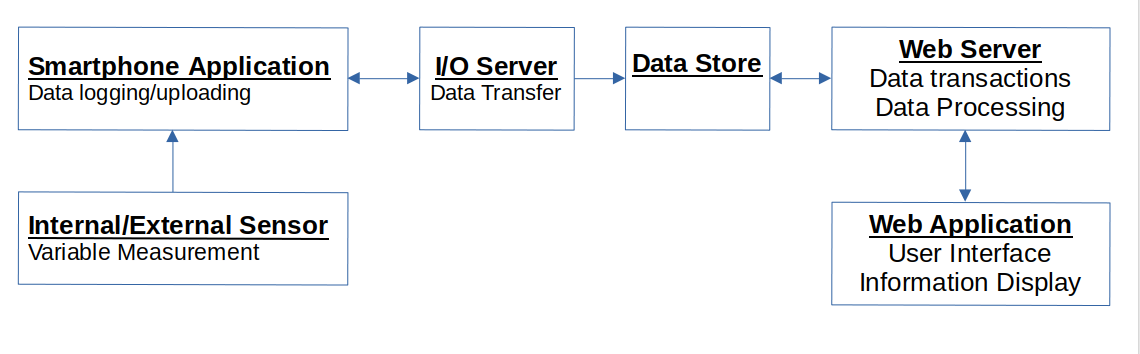
\includegraphics[scale=0.45]{high_arch.png}
    \caption{Proposed High Level Architecture}
    \label{fig:high_arch}
\end{figure}

\subsection{Project Objective}
\subsubsection{Primary Objective}
The primary objective in addressing the problem will be the development of detailed reports showcasing the trucker's whereabouts and behavior during their work shifts.

\subsection{Anticipated Benefits of Solution}
Managers will be able to ensure that their truckers conduct their work efficiently and responsibly.
They will then be able to adequately handle truckers who fail to perform as expected.

Managers may also be able to analyze trucker behavior to perform optimizations, potentially allowing for increased efficiency.

\subsection{Technical Requirements}
A set of requirements are identified in realizing the hypothesized solution and the scope is identified. 

\subsubsection{Requirements}
\begin{enumerate}
\item \textbf{Smartphone Application}\\
    This will be a smartphone application used by the entities being tracked(i.e the truckers).
    \begin{enumerate}
        \item Trucker identification control must be implemented to ensure that logs sent to the server correspond to a unique trucker. It must not be possible for multiple truckers to assume the same or no identity.
        \item Every 2 minutes, sensor data capturing the \textbf{\ac{gps} coordinates, altitude, speed and acceleration} must be captured and stored internally on the android device. 
        Data capacity for one continuous week of storage must be possible, to account for connectivity issues.
        \item The application must be able to run in the background, allowing for multitasking.
        \item Sensor data must be uploaded to a central data store, either continuously or on request. This communication must be encrypted for security purposes.
    \end{enumerate}
\item \textbf{\ac{io} Server}\\
This server will facilitate the transfer of logged data from the Smartphone Application to a central data store, via an internet connection. 
    \begin{enumerate}
        \item As a dedicated transfer server, it must exhibit high performance, handling multiple requests from the multiple smartphone clients asynchronously.
        \item Trucker logs, received from smartphone clients, must be stored in a central database.
        \item Information about the trucking company must also be sent to the smartphone client.
    \end{enumerate}
\item \textbf{Data Store}\\
The data store will be efficient, fast and capable of storing large volumes of data.
It should also be capable of adequately interfacing with the \ac{io} server and the Web Server.
The web server is responsible for querying data from the data store, and serving requests to the web application.
\item \textbf{Web Server and Web Application}\\
The web server must implement back-end business logic and serve pages in the web application.
The web application acts as an interface for managers to add truckers and view tracking information about their fleets.
    \begin{enumerate}
        \item Multiple trucking managers must be able to log in and use the application.
        \item Managers must be able to add multiple truckers to their fleet, including trucker-specific information such as name, and vehicle number.
        \item Managers must be able to view detailed trip information for any adjustable time period. Log data must be processed to determine starting and arrival times for locations traveled to. Statistical information about acceleration and speed should be displayed, including averages, maximums and percentiles.
    \end{enumerate}
\end{enumerate}
\subsubsection{Scope Definition}
The scope of the problem considered will include
\begin{enumerate}
\item \textbf{Internal/External Sensor Interface}\\
The scope \textbf{does not} include the design of sensor circuitry meant to interface with the smartphone. Only configurations capable of interfacing with the smartphone are considered.
The smartphone app is not concerned with displaying user reports and statistics. That is left to the web application.
\item \textbf{Smartphone Application}\\
The smartphone application is purely responsible for logging the appropriate sensor data and transferring the sensor data on through the \ac{io} server.
Other measurable variables such as temperature, fuel and pressure are not considered.
\item \textbf{\ac{io} Server}\\
The \ac{io} server is purely responsible for facilitating the transfer of sensor data from the smartphone to the data store.
\item \textbf{Data Store}\\
    The data store element is purely concerned with the storage of logs, user identity information and providing an interface for the \ac{io} server to query and add records to the store.
    Existing data store providers will be considered.
\end{enumerate}

\subsection{Deliverables}
The deliverables will require the entire project to function, from the smartphone logging implementation, to the detailed reports available in the web application. 
\begin{itemize}
\item Smartphone Application and \ac{io} server
\item Web Application and web server
\end{itemize}

\subsection{Conclusion}
Basic contextualization of the problem has been performed.
Low level details, however, have not been considered.
Each aspect of the planned architecture may be realized in multiple ways on the low level.
Further research and a feasibility analysis are necessary for adequate low level design.

\pagebreak
